% Drawing 138/07-5 -- folder 138, batch 07, archive page 126 (PDF page 127).
% Transcription: une sphère vue en coupe, portant les points $0$ (en haut), $1$ (en bas), $\infty$ et $\tfrac12$ sur deux méridiens ; un triangle découpé en cases.
% Kind: sphere with meridians; triangle cut into cells. Method 2 (schematic redraw from the facsimile). Status: partial.
% Notes: A sphere seen in section: 0 at the top, 1 at the bottom, two meridians, infinity and 1/2 on them (the 1/2 reads « 1/3 » on the page, hard to tell). A triangle cut into cells by inner strokes; the cells are small loops and strokes that are only roughly drawn. A second sphere with 0, 1, infinity lower on the page, among the matrix computations, is not covered by this mark and not drawn. The page also carries doodles (a figure in a triangle, a profile with a hat) that the transcription mentions in a note and that no mark covers; they are not drawn.
% Coordinates: 1 unit = 1 mm = 1/100 of the crop width (bbox in page fractions: [0.114, 0.113, 0.408, 0.238]).
% Redrawn by Claude (claude-opus-5-5), issue #73, 2026-11-07; not checked by a human; not compiled (no TeX in the session).
% Rights: reproduces part of the work -- behind RENDER_TRANSCRIPTS, never published by itself.
\documentclass[tikz,border=3pt]{standalone}
\usepackage{amsmath,amssymb}
\usetikzlibrary{patterns,arrows.meta}
\tikzset{pencil/.style={black!45}, struck/.style={black!35}, mark/.style={circle,draw,inner sep=1.3pt}, pt/.style={circle,fill,inner sep=0.9pt}, opt/.style={circle,draw,fill=white,inner sep=1.1pt}}
\begin{document}
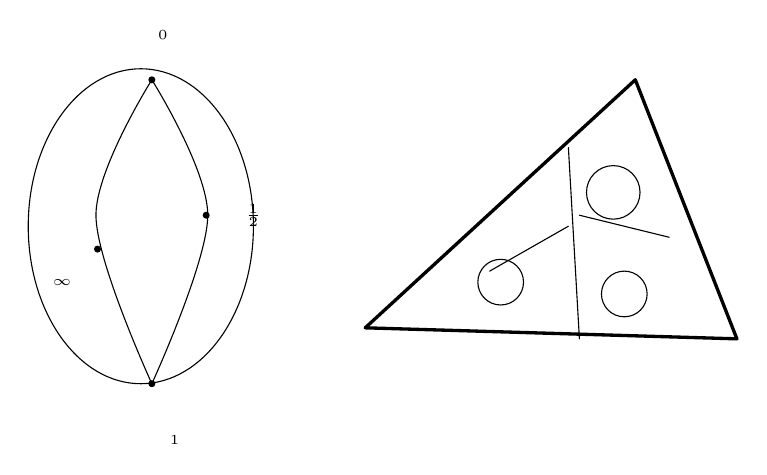
\begin{tikzpicture}[x=1mm,y=1mm,line cap=round,line join=round,font=\scriptsize]
\draw (18.6,-30) ellipse[x radius=14.3, y radius=20];
\draw plot[smooth, tension=0.55] coordinates {(20,-11.4) (12.9,-28.6) (20,-50)};
\draw plot[smooth, tension=0.55] coordinates {(20,-11.4) (27.1,-28.6) (20,-50)};
\node[pt] at (20,-11.4) {};
\node[pt] at (20,-50) {};
\node[pt] at (13.1,-32.9) {};
\node[pt] at (26.9,-28.6) {};
\node[inner sep=1pt] at (21.4,-5.7) {\tiny $0$};
\node[inner sep=1pt] at (22.9,-57.1) {\tiny $1$};
\node[inner sep=1pt] at (8.6,-37.1) {\tiny $\infty$};
\node[inner sep=1pt] at (32.9,-28.6) {\tiny $\frac12$};
\draw[very thick] (47.1,-42.9) -- (81.4,-11.4) -- (94.3,-44.3) -- cycle;
\draw (72.9,-20) -- (74.3,-44.3);
\draw (62.9,-35.7) -- (72.9,-30);
\draw (74.3,-28.6) -- (85.7,-31.4);
\draw (64.3,-37.1) circle[radius=2.9];
\draw (78.6,-25.7) circle[radius=3.4];
\draw (80,-38.6) circle[radius=2.9];
\end{tikzpicture}
\end{document}
